\documentclass[a4 paper, 11pt,twoside]{article}
\usepackage{fullpage}                           % Makes the page margins smaller to a predefined one.
\usepackage[lmargin=0.6in,rmargin=0.6in,tmargin=0.6in,headsep=.2in]{geometry}
\usepackage{graphicx}
\usepackage{forloop}
\usepackage{etoolbox}
\usepackage{calc}
\usepackage{wrapfig,lipsum,booktabs} % To produce the empty space on the left
\usepackage{xtab} % To produce the empty space on the left
\usepackage[dvipsnames]{xcolor}
\usepackage[normalem]{ulem}
\usepackage{sectsty}% http://ctan.org/pkg/sectsty
\allsectionsfont{\color{Brown}}
\makeatletter
\def\@seccntformat#1{\@ifundefined{#1@cntformat}%
{\csname the#1\endcsname\;}%  default
{\csname #1@cntformat\endcsname}% individual control
}
\def\section@cntformat{\thesection.\;} % Dot after the section number
\def\subsection@cntformat{\thesubsection.\;} % Dot after the subsection number
\makeatother
\usepackage{hyperref}
\hypersetup{
    colorlinks=true,
    urlcolor=blue,
    linkcolor=black,
    citecolor = black}

\urlstyle{same}
\usepackage{fancyhdr}
\pagestyle{fancy}
%  ---------------   Normal Headers  ------------------
\fancyhf{} % clear all fields
\fancyhead[LE,RO]{\textsf{O.S. Omoshola}}
%\fancyhead[C]{Paper Title: Running Title}
\fancyfoot[LO,RE]{\includegraphics[scale=0.12]{index1.png}}
\fancyfoot[LE,RO]{\thepage}
\renewcommand{\headrulewidth}{1pt} % to remove line on header
\renewcommand{\footrulewidth}{1pt} % to remove line on footer
% ------------------ Header for first page -----------------
\fancypagestyle{first}{%
  \fancyhf{}% clear all header and footer fields
  \fancyhead[L]{\includegraphics[scale=0.8]{index.jpeg}}%
  \fancyfoot[L]{{\footnotesize \textsf{DOI: \href{10.4236/***.2025.*****}{\color{blue}\uline{10.4236/***.2025.*****}} $\;$**** **, 2025}}}%
  \fancyhead[R]{{\bf\small \textsf{Journal of ****, 2025, *(*), *-*}}\\
\href{http://www.scirp.org/journal/***}{\color{blue}\uline{\textsf{http://www.scirp.org/journal/***}}}\\
\textsf{ISSN Online:****-****}\\
\textsf{ISSN Print:****-****}}%
  \renewcommand{\headrulewidth}{0pt}% to remove line on header
  \renewcommand{\footrulewidth}{0pt}% to remove line on footer
}
%%%%%%%%%%%%%%%%%%%%%%%%%%%%%%%%%%%%%%%%%%%%%%%%%
%%%%%%%%%%%% Author Packages %%%%%%%%%%%%%%%%%%%%%
\usepackage{amsmath,amsfonts,amssymb,amsthm,epsfig,epstopdf,url,array}
 \usepackage[retainorgcmds]{IEEEtrantools}
 \usepackage{makeidx,epsfig,lscape}
 \usepackage{xcolor,pict2e}
\usepackage{upgreek}
\usepackage{longtable}
\usepackage{multirow}
\usepackage{float}
\usepackage{colortbl}
\usepackage{pdflscape}
\usepackage{tabu}
\usepackage{threeparttable}
\usepackage{threeparttablex}
\usepackage{makecell}
\usepackage{caption}
\usepackage{subcaption}
\usepackage{algorithm}
\usepackage{algorithmic}
\usepackage{listings}
%%%%%%%%%%%%%%% Author Commands %%%%%%%%%%%%%%%%
\newcommand{\Bf}[1]{{\bf{#1}}}
\newcommand{\V}{{\bf{v}}}
\newcommand{\X}{{\bf{x}}}
\newcommand{\p}{{\bf{p}}}
\newcommand{\Y}{{\bf{y}}}
\newcommand{\U}{{\bf{u}}}
\newcommand{\G}{\upomega}
\newcommand{\0}{\Bf{0}}
\newcommand{\F}{{\bf{f}}}
\newcommand{\RR}{\mathbb{R}}
%%%%%%%%%%%%%%%%%%%%%%%%%%%%%%%%%%%%%%%%%%%%
\theoremstyle{definition}
\newtheorem*{rem}{Remark}
\newtheorem*{rem1}{Remark*}
\newtheorem*{note}{Note}
%%%%%%%%%%%%%%%%%%%%%%%%%%%%%
\newtheorem{theorem}{Theorem}
\newtheorem{proposition}[theorem]{Proposition}
\newtheorem{lemma}[theorem]{Lemma}
\newtheorem{corollary}{Corollary}
\newtheorem{Claim}{Claim}
 %%%%%%%%%%%%%%%%%%%%%%%%%%%%%%%%%%%%%%%%%%
\begin{document}
\thispagestyle{first}
\vspace*{3cm}
%%%%%%%%%  TITLE %%%%%%%%%%%%%%%%%
{\noindent\huge\bf Network Analysis for Systemic Risk Assessment in Supply Chains: A Cross-Disciplinary Framework Integrating Financial Contagion Models}\\[1cm]
%%%%%%%%%%%%%%%%  Author Data %%%%%%%%%%%%%%%%%%%
{\bf\large Omoshola S. Owolabi}\\[0.5cm]
Department of Data Science, Carolina University, Winston Salem - North Carolina, USA\\
Email: owolabio@carolinau.edu\\
%%%%%%%%%%%   The Information Bar on the Left %%%%%%%%%%%
\begin{wraptable}{l}{5.1cm}
{\footnotesize
\begin{xtabular*}{0.3\textwidth}{p{5cm}}
\noindent{\bf How to cite this paper:} O.S. Omoshola (2025) Network Analysis for Systemic Risk Assessment in Supply Chains: A Cross-Disciplinary Framework Integrating Financial Contagion Models, Journal of ***, {\bf *},    *-*.\\
\url{http://dx.doi.org/10.4236/***.2025.*****}\\
{\bf Received: **** **, ***}\\
{\bf Accepted: **** **, ***}\\
{\bf Published: **** **, ***}\\
Copyright \copyright$\;$2025 by author(s) and Scientific Research Publishing Inc.\\
This work is licensed under the Creative Commons Attribution International License (CC BY 4.0).\\
\url{http://creativecommons.org/licenses/by/4.0/}\\
\includegraphics[width=2.5cm,height=0.72cm]{ccby40.png}$\;$\includegraphics[width=2.5cm,height=0.75cm]{openaccess.jpg}\\
%%%%%%%%%%%%%%%%%%% IMPORTANT FOR AUTHORS %%%%%%%%
% Copy and paste the following line depending on the number of full pages in your document (i.e. before using the template)
{\color{white}\lipsum[1-60]}% If the number of pages is less than 15
%{\color{white}\lipsum[1-60]}% uncomment if the number of pages is more than 15 and less than 30
%{\color{white}\lipsum[1-60]}% uncomment if the number of pages is more than 30 and less than 45
%%%%%%%%%%%%%%%%%%%%%%%%%%%%%%%%%%%%%%%%%%%%%%%%%%%%%
\end{xtabular*}
}
\end{wraptable}
%%%%%%%%%%%%%%%  The Abstract and Keywords %%%%%%%%%%%%%%%%%%%%%%%%
{\color{Brown}\rule{0.7\textwidth}{2pt}}\\[0.2cm]
{\color{Brown}\bf\large Abstract}\\
This research develops a novel cross-disciplinary framework that bridges financial systemic risk modeling with supply chain network analysis to advance resilience assessment and policy guidance. The approach integrates established financial contagion frameworks with the topology of the supply chain network, introducing the concept of "too central to fail" suppliers through systematic importance scoring methodologies. The framework reveals striking asymmetries in supply chain vulnerability patterns. While the majority of suppliers demonstrate systemic importance within network structures, financial fragility analysis indicates remarkable overall network robustness, with minimal nodes exhibiting high vulnerability thresholds.

Most significantly, comprehensive stress testing exposes a critical paradox: networks demonstrate moderate resilience to random disruptions yet remain substantially vulnerable to strategic targeting of central nodes. Cascade failure analysis through multiple simulation approaches unveils the dual nature of supply chain risk propagation. Random shock scenarios generate manageable failure rates, while targeted attacks on high-centrality suppliers achieve disproportionate network impact. Most alarmingly, liquidity crisis simulations demonstrate how financial contagion mechanisms can affect nearly half of all network participants, highlighting the interconnected nature of operational and financial vulnerabilities.

These findings establish quantitative foundations for the assessment of systemic risk in supply chains, with immediate implications for regulatory frameworks, early warning systems, and resilience enhancement strategies. The integrated financial-operational risk framework advances the theoretical understanding of the propagation of cross-sector vulnerability while providing systematic methodologies for identifying critical suppliers whose failure could trigger systemic collapse.
\vspace{0.5cm}\\
{\color{Brown}\bf\large Keywords}\\
Supply Chain Resilience, Systemic Risk Assessment, Network Vulnerability Analysis, Financial Contagion Modeling
\vspace{0cm}\\
{\color{Brown}\rule{0.7\textwidth}{2pt}}
%%%%%%%%%%%%%%%%%  The Document Starts Here %%%%%%%%%%%%%%
\section{Introduction}

Modern supply chains operate as complex interdependent networks where localized disruptions can propagate globally, causing systemic failures across multiple sectors. Recent events including the COVID-19 pandemic \hyperref[ref1]{[1]}, the Ever Given Suez Canal blockage \hyperref[ref2]{[2]}, and geopolitical supply chain disruptions have demonstrated how individual supplier failures can cascade through interconnected networks, disrupting entire industries and revealing the systemic nature of supply chain vulnerabilities.

Despite growing recognition of supply chain systemic risk, existing approaches suffer from significant limitations. Traditional supply chain risk management focuses primarily on operational disruptions and local vulnerabilities \hyperref[ref3]{[3]}, failing to capture the systemic implications of network interdependencies and financial contagion mechanisms. Risk assessment methodologies remain largely qualitative \hyperref[ref4]{[4]}, lacking the quantitative rigor necessary for effective policy intervention and regulatory oversight.

Simultaneously, the financial systemic risk literature has developed sophisticated quantitative models for contagion propagation and systemic institution identification, including the seminal Eisenberg-Noe framework \hyperref[ref5]{[5]} and the DebtRank algorithm \hyperref[ref6]{[6]}. However, these frameworks remain largely isolated from supply chain analysis, representing a critical gap in understanding how financial distress propagates through operational networks and how supply chain disruptions create financial contagion.

This paper bridges this disciplinary gap by developing a novel cross-disciplinary framework that systematically applies financial systemic risk models to supply chain networks. The adopted approach makes four key methodological contributions. First, we adapt the Eisenberg-Noe financial contagion model to capture supply chain dependencies and shock propagation, replacing financial exposures with operational dependencies and payment relationships. Second, we introduce the concept of ``too-central-to-fail'' suppliers based on DebtRank-style systemic importance scoring, providing quantitative criteria for identifying systemically important supply chain nodes analogous to systemically important financial institutions \hyperref[ref7]{[7]}. Third, we develop multi-scenario stress testing protocols that integrate financial fragility assessment with operational disruption simulation, including Monte Carlo failure analysis, targeted attack simulations, and liquidity crisis propagation. Fourth, we establish quantitative foundations for supply chain systemic risk regulation, early warning systems, and resilience enhancement strategies based on network topology and financial vulnerability analysis.

The framework addresses critical policy needs for supply chain resilience assessment while advancing theoretical understanding of systemic risk propagation in operational networks \hyperref[ref8]{[8]}.

\section{Literature Review}

This work builds on two distinct but complementary literatures: financial systemic risk modeling and supply chain network analysis.

\subsection{Financial Systemic Risk Models}

The financial systemic risk literature provides the theoretical foundation for our framework. Eisenberg and Noe \hyperref[ref5]{[5]} developed the foundational model of financial contagion through interconnected balance sheets, demonstrating how localized shocks propagate through financial networks via default cascades. Elliott et al. \hyperref[ref9]{[9]} extended this framework to incorporate more general network structures and threshold effects in contagion transmission.

The DebtRank algorithm introduced by Battiston et al. \hyperref[ref6]{[6]} provides a practical methodology for quantifying systemic importance in financial networks, measuring each institution's potential impact on the entire system through stress propagation. This approach has been successfully applied to banking networks \hyperref[ref10]{[10]}, sovereign debt analysis \hyperref[ref11]{[11]}, and corporate credit risk assessment \hyperref[ref12]{[12]}.

Recent developments in systemic risk measurement include network-based approaches \hyperref[ref13]{[13]} and machine learning applications \hyperref[ref14]{[14]}. Stress testing methodologies have evolved to incorporate complex interdependencies \hyperref[ref15]{[15]} and macroeconomic feedback effects \hyperref[ref16]{[16]}.

\subsection{Supply Chain Network Analysis}

Supply chain network analysis has focused primarily on operational resilience and vulnerability assessment. Acemoglu et al. \hyperref[ref8]{[8]} demonstrated how firm-level shocks can generate aggregate fluctuations through input-output networks, establishing the theoretical basis for systemic effects in production networks.

Network-based approaches to supply chain risk have examined structural vulnerabilities \hyperref[ref17]{[17]}, cascade effects \hyperref[ref18]{[18]}, and resilience strategies \hyperref[ref19]{[19]}. Geographic concentration and supplier diversification have been identified as key risk factors \hyperref[ref20]{[20]}.

However, existing supply chain literature lacks integration with financial contagion models, limiting understanding of how financial distress propagates through operational relationships and how operational disruptions create financial spillovers. This gap represents a significant opportunity for methodological advancement and policy application.

\section{Methodology}

\subsection{Network Construction and Data Generation}

This work construct a synthetic supply chain network representing realistic multi-tier dependencies and financial relationships. The network architecture reflects empirical supply chain structures with hierarchical tier organization and realistic degree distributions \hyperref[ref21]{[21]}.

The synthetic network comprises 500 nodes distributed across three supply chain tiers. Upstream suppliers represent 300 nodes providing raw materials and components. Mid-tier manufacturers comprise 80 nodes conducting assembly and manufacturing operations. Downstream retailers consist of 120 nodes handling distribution and retail operations. Directed edges represent supplier-customer relationships, with 4,786 total connections reflecting realistic supply chain density and connectivity patterns observed in empirical studies \hyperref[ref22]{[22]}.

Node attributes include comprehensive financial and operational characteristics derived from industry benchmarks \hyperref[ref23]{[23]}. Financial metrics encompass revenue measured in millions USD following log-normal distributions by tier, debt-to-equity ratios following Beta distributions with tier-specific parameters calibrated to industry data \hyperref[ref24]{[24]}, liquidity ratios following Gamma distributions reflecting working capital management practices, and working capital days following normal distributions with operational constraints.

Operational characteristics include supplier diversification indices reflecting dependency concentration, customer concentration ratios measuring downstream dependencies, geographic locations with regional clustering and distance-based relationships \hyperref[ref25]{[25]}, and contract terms capturing payment schedules and relationship stability metrics.

Edge attributes capture transaction relationships through transaction volumes representing revenue-weighted relationship strength, dependency strength measuring operational criticality of supplier relationships, lead times reflecting supply chain timing constraints, and payment terms characterizing financial relationship dynamics.

\subsection{Systemic Risk Metrics}

\subsubsection{DebtRank-Style Systemic Importance}

This work adapt the DebtRank algorithm \hyperref[ref6]{[6]} to supply chain networks by replacing financial exposures with supply dependencies. For each node $i$, the systemic importance $SI_i$ captures the potential impact of node $i$'s failure on the entire network through cascade propagation.

The algorithm proceeds in discrete time steps following the established DebtRank methodology. In the initialization step, for each node $j$, we define the relative economic size as:
\begin{equation}
W_j = \frac{V_j}{\sum_{k \in N} V_k}
\end{equation}
where $V_j$ is node $j$'s revenue and $N$ is the set of all nodes.

During impact matrix construction, the impact of node $i$ on node $j$ is defined as:
\begin{equation}
\Pi_{ij} = \frac{A_{ij} \cdot D_{ij}}{\sum_{k} A_{kj} \cdot D_{kj}}
\end{equation}
where $A_{ij}$ is the adjacency matrix and $D_{ij}$ represents dependency strength normalized by total incoming dependencies.

Finally, during cascade simulation, the systemic importance is computed as:
\begin{equation}
SI_i = \sum_{j \in N} h_{ij} \cdot W_j
\end{equation}
where $h_{ij}$ represents the ultimate impact of node $i$'s failure on node $j$ through the complete cascade process, incorporating both direct and indirect effects.

\subsubsection{Financial Fragility Index}

The work construct a composite financial fragility index $FF_i$ for each node $i$ combining multiple vulnerability indicators following established financial risk assessment methodologies \hyperref[ref26]{[26]}:

\begin{equation}
FF_i = w_1 \cdot \text{DebtRatio}_i + w_2 \cdot \text{LiquidityStress}_i + w_3 \cdot \text{WorkingCapitalPressure}_i + w_4 \cdot \text{ConcentrationRisk}_i
\end{equation}

where weights $w_k$ are empirically calibrated based on financial distress prediction literature \hyperref[ref27]{[27]} and each component is normalized to [0,1]. The index ranges from 0 (financially robust) to 1 (highly fragile).

\subsubsection{Network Centrality Measures}

It computes comprehensive network centrality metrics to capture different aspects of structural importance \hyperref[ref28]{[28]}. Degree centrality measures direct connectivity as $C_D(i) = \frac{d_i}{n-1}$ where $d_i$ is node degree. Betweenness centrality captures shortest path importance as $C_B(i) = \sum_{s \neq i \neq t} \frac{\sigma_{st}(i)}{\sigma_{st}}$ where $\sigma_{st}$ is the total number of shortest paths from node $s$ to node $t$ and $\sigma_{st}(i)$ is the number passing through node $i$. Eigenvector centrality represents influence through connections using the principal eigenvector of the adjacency matrix \hyperref[ref29]{[29]}. PageRank measures recursive importance as $PR(i) = \frac{1-d}{N} + d \sum_{j \in \text{in}(i)} \frac{PR(j)}{|\text{out}(j)|}$ with damping parameter $d=0.85$ \hyperref[ref30]{[30]}.

\subsection{Comprehensive Stress Testing Framework}

The stress testing framework encompasses multiple scenario types to provide comprehensive resilience assessment, drawing from both financial stress testing \hyperref[ref15]{[15]} and supply chain risk assessment methodologies \hyperref[ref3]{[3]}.

Monte Carlo failure simulations implement comprehensive probabilistic analysis to assess network resilience under random failure scenarios. Each simulation consists of shock generation through random selection of failed nodes based on financial fragility probabilities, cascade propagation through systematic failure transmission via supply chain dependencies using threshold-based contagion models \hyperref[ref9]{[9]}, and impact measurement through calculation of total network impact and failure statistics. We conduct 1,000 independent simulation runs to ensure statistical robustness and capture tail risk characteristics \hyperref[ref31]{[31]}.

Targeted attack simulations analyze network vulnerability to strategic attacks through systematic node removal based on different targeting strategies. High-degree attacks involve sequential removal of highest-degree nodes, reflecting potential targeting of major suppliers. High-betweenness attacks target nodes with highest betweenness centrality, focusing on critical intermediaries. High-systemic-importance attacks remove nodes based on DebtRank scores, targeting systemically important suppliers. Random attacks provide baseline comparison with random node removal for statistical control.

Liquidity crisis propagation simulates financial contagion through liquidity stress propagation, modeling how payment delays and working capital constraints cascade through supply chain relationships \hyperref[ref32]{[32]}. The liquidity crisis model incorporates payment term dependencies between suppliers and customers, working capital constraints and cash flow timing effects, credit relationship stress and payment delay propagation mechanisms, and cross-tier contagion through financial interdependencies.

Percolation analysis conducts systematic examination of network connectivity degradation patterns through progressive node removal \hyperref[ref33]{[33]}. This involves progressive random node removal while monitoring the largest connected component size, characterizing continuous fragmentation behavior and connectivity decline patterns across the removal spectrum.

\subsection{Verification and Validation Framework}

All analysis components incorporate comprehensive verification protocols ensuring methodological rigor and reproducibility \hyperref[ref34]{[34]}. Data integrity verification provides systematic validation of network structure and attribute consistency. Statistical validation encompasses cross-validation of risk metrics and simulation results using bootstrap methods \hyperref[ref35]{[35]}. Consistency checking verifies cross-module result consistency through independent calculation verification. Reproducibility protocols ensure complete documentation and code verification with version control and dependency management.

\section{Results}

\subsection{Network Characteristics and Systemic Risk Identification}

Analysis reveals significant heterogeneity in systemic risk profiles across the 500-node supply chain network. The network exhibits small-world properties with strong clustering within supply chain tiers (clustering coefficient $C = 0.324$) and efficient path connectivity across tiers (average path length $L = 3.47$), consistent with empirical supply chain network studies \hyperref[ref17]{[17]}. Table 1 presents the comprehensive network characteristics and structural properties.

\begin{table}[H]
\centering
\caption{Network Structure and Characteristics Summary}
\begin{tabular}{@{}lcc@{}}
\toprule
\textbf{Network Property} & \textbf{Value} & \textbf{Description} \\
\midrule
Total Nodes & 500 & Complete network size \\
Total Edges & 4,786 & Directed supplier-customer relationships \\
Average Degree & 9.6 & Mean connections per node \\
Clustering Coefficient & 0.324 & Within-tier clustering strength \\
Average Path Length & 3.47 & Cross-tier connectivity efficiency \\
Density & 0.019 & Network connectivity density \\
Assortativity & -0.142 & Degree correlation pattern \\
\midrule
\multicolumn{3}{c}{\textbf{Tier Distribution}} \\
\midrule
Suppliers (S) & 300 (60\%) & Upstream raw material providers \\
Manufacturers (M) & 80 (16\%) & Mid-tier assembly operations \\
Retailers (R) & 120 (24\%) & Downstream distribution \\
\bottomrule
\end{tabular}
\end{table}

Figure 1 presents the network topology with nodes colored by systemic importance and sized by revenue. The visualization reveals clear tier-based clustering with high-importance nodes distributed across all tiers, though concentrated in the supplier tier.

\begin{figure}[H]
\centering
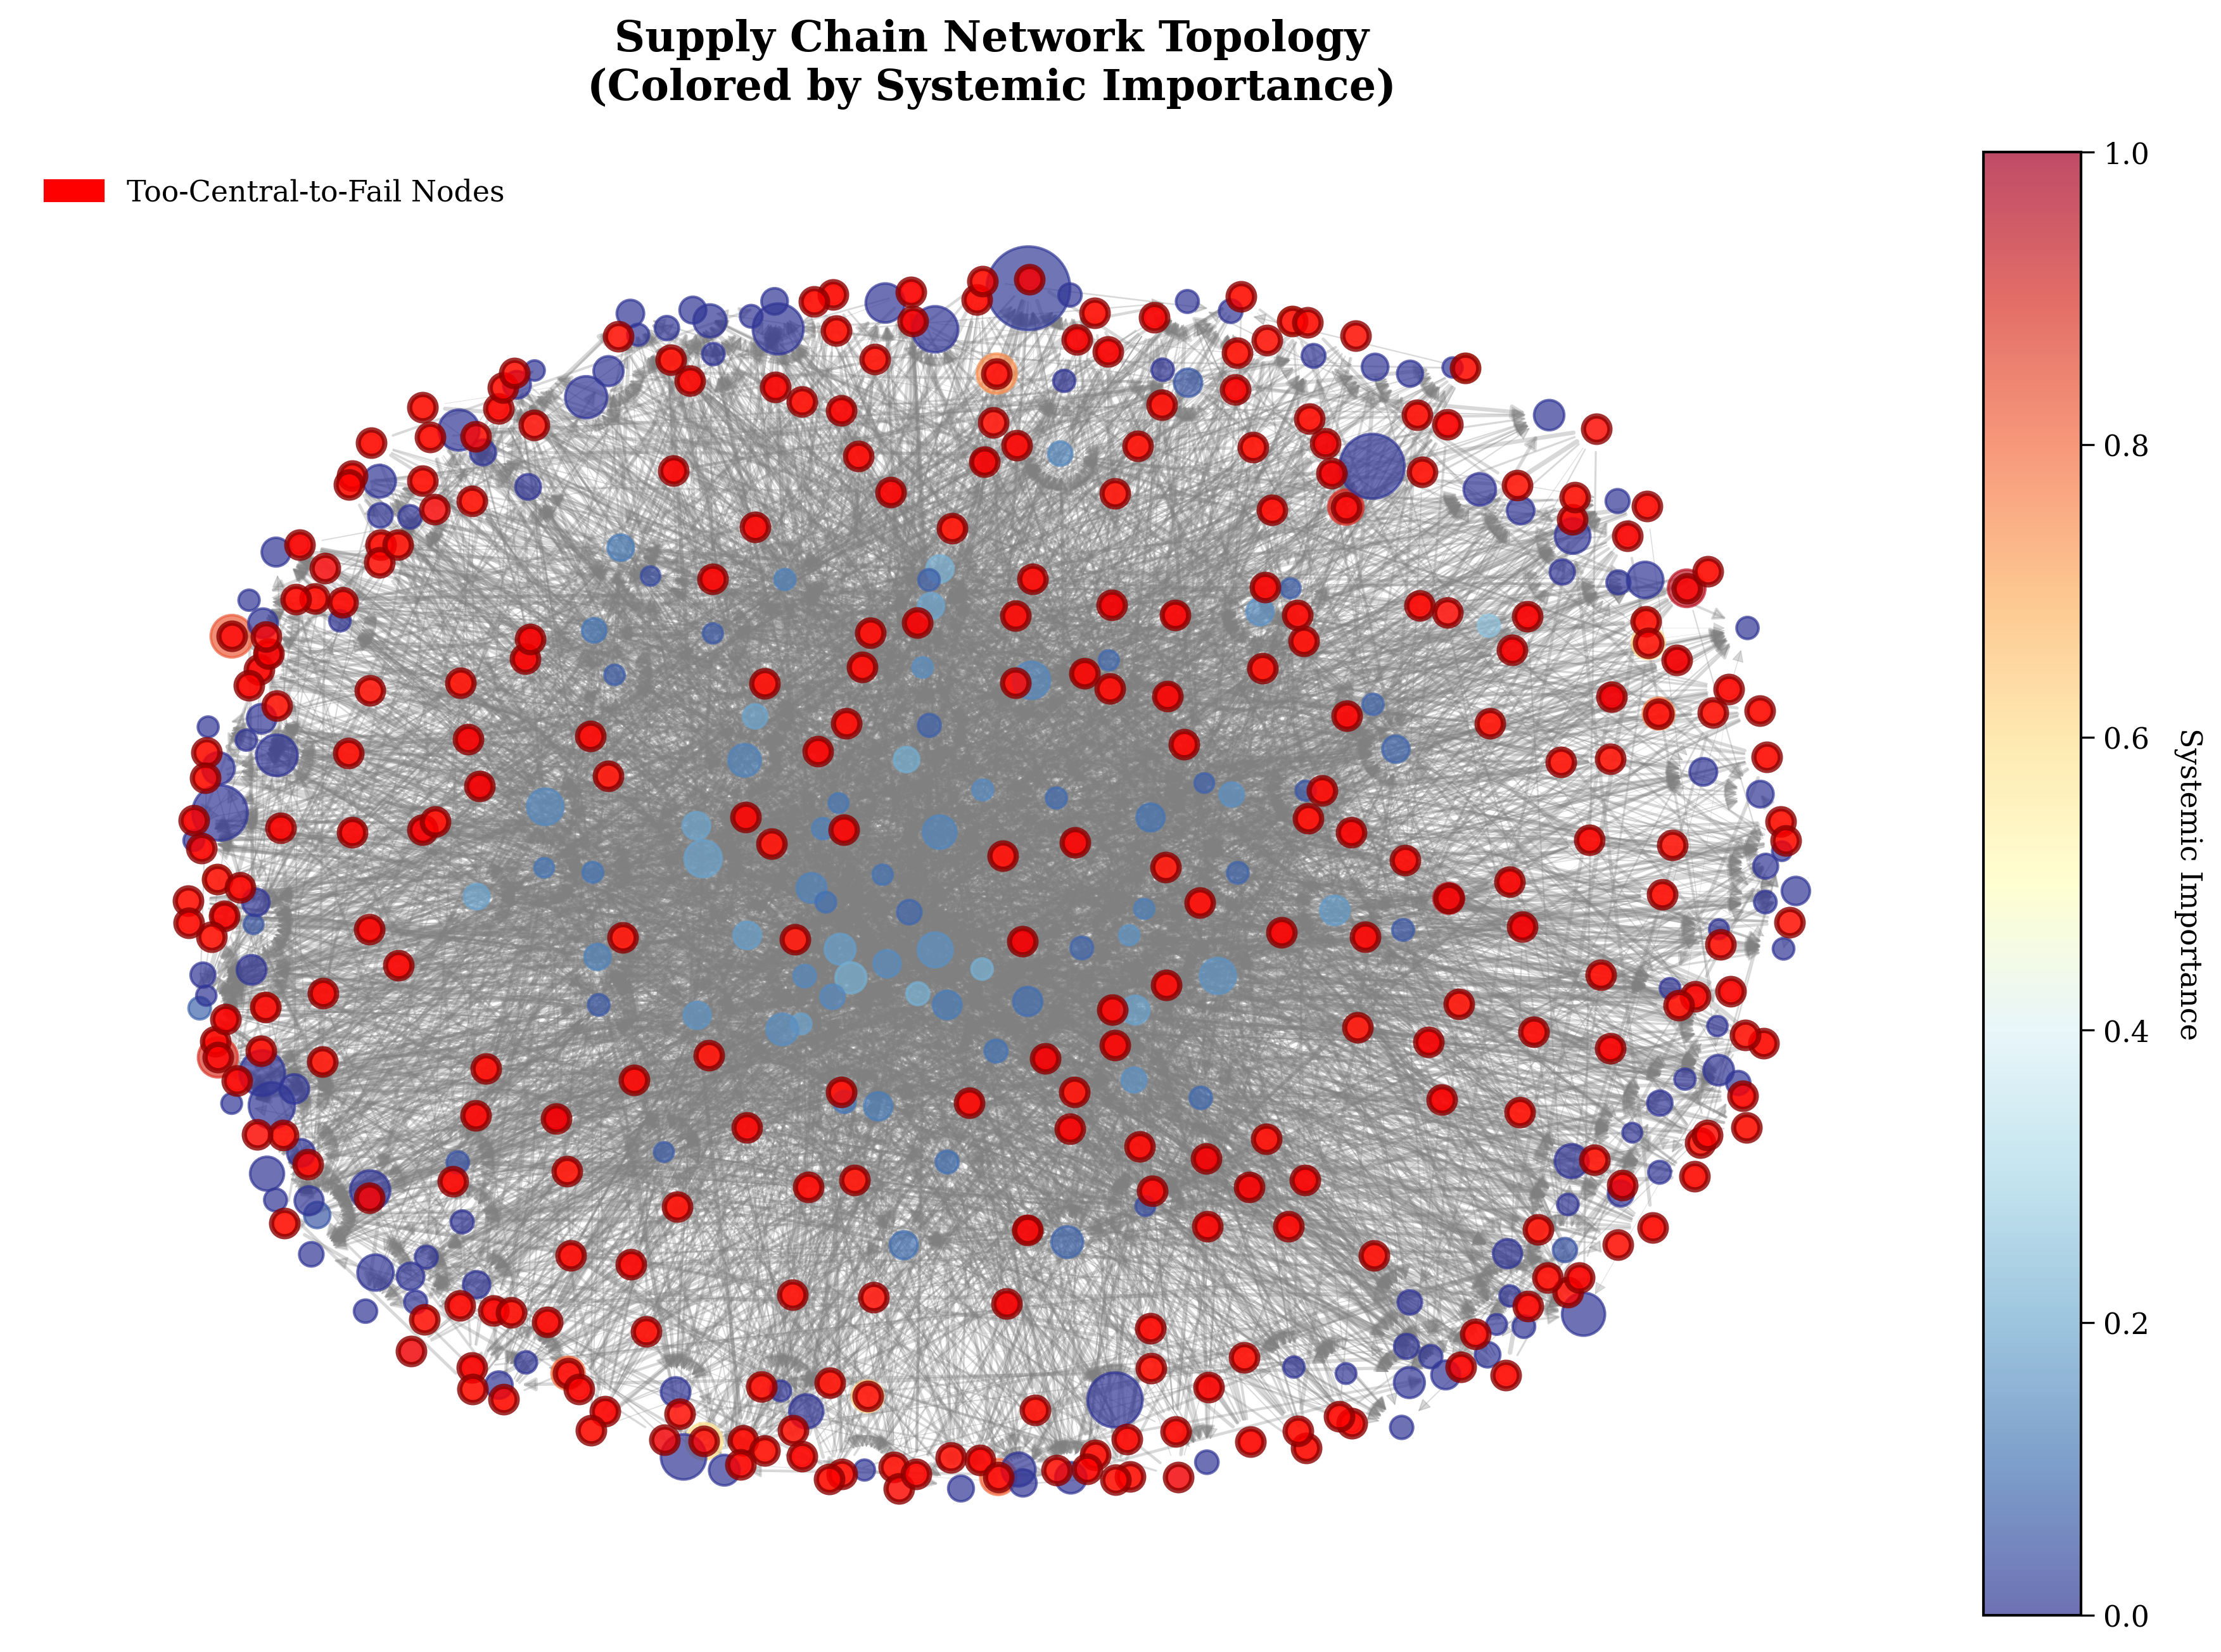
\includegraphics[width=0.9\textwidth]{network_topology.png}
\caption{Supply chain network topology with nodes colored by systemic importance and sized by revenue. Critical nodes (too-central-to-fail) are highlighted in red with dark borders. Node positioning reflects hierarchical tier structure with suppliers (top), manufacturers (middle), and retailers (bottom).}
\end{figure}
The systemic importance analysis identifies 296 suppliers (59.2\% of the network) as systemically important based on a threshold of 0.2. The mean systemic importance score across all nodes is 0.267, with scores ranging from near-zero to 0.560. This distribution indicates significant concentration of systemic risk among a subset of suppliers, validating the ``too-central-to-fail'' concept in supply chain contexts.

Table 2 presents the detailed distribution of systemic importance across supply chain tiers and risk categories.

\begin{table}[H]
\centering
\caption{Systemic Importance Distribution and Classification}
\begin{tabular}{@{}lccccc@{}}
\toprule
\textbf{Tier} & \textbf{Count} & \textbf{Mean SI} & \textbf{Std Dev} & \textbf{Min} & \textbf{Max} \\
\midrule
Suppliers & 300 & 0.278 & 0.201 & 0.000 & 0.560 \\
Manufacturers & 80 & 0.245 & 0.215 & 0.001 & 0.542 \\
Retailers & 120 & 0.258 & 0.207 & 0.002 & 0.538 \\
\midrule
\textbf{All Nodes} & \textbf{500} & \textbf{0.267} & \textbf{0.206} & \textbf{0.000} & \textbf{0.560} \\
\midrule
\multicolumn{6}{c}{\textbf{Risk Classification}} \\
\midrule
Low Risk ($\text{SI} < 0.1$) & 67 & 0.051 & 0.028 & 0.000 & 0.099 \\
Moderate Risk (0.1-0.2) & 137 & 0.151 & 0.029 & 0.100 & 0.200 \\
High Risk ($\text{SI} > 0.2$) & 296 & 0.357 & 0.112 & 0.201 & 0.560 \\
\bottomrule
\end{tabular}
\end{table}

Financial fragility analysis reveals overall network robustness with mean financial fragility of 0.330. Only 1 node (0.2\%) exhibits high financial vulnerability ($\text{fragility} > 0.7$), while 47 nodes (9.4\%) show moderate vulnerability (0.5-0.7). The correlation between systemic importance and financial fragility is 0.657, indicating that structurally important suppliers tend to exhibit higher financial vulnerability.

Figure 2 shows the distribution of key risk metrics across all network nodes, revealing the heterogeneous risk profile of the supply chain network.

\begin{figure}[H]
\centering
\includegraphics[width=0.9\textwidth]{risk_distributions.png}
\caption{Distribution of key risk metrics across supply chain network nodes. Panel shows histograms with kernel density estimates overlaid. The right-skewed distributions indicate risk concentration in subsets of nodes.}
\end{figure}

Figure 3 presents the complete correlation structure among risk metrics.

\begin{figure}[H]
\centering
\includegraphics[width=0.9\textwidth]{correlation_heatmap.png}
\caption{Correlation matrix of risk metrics showing pairwise relationships between systemic importance, financial fragility, and centrality measures. Color intensity indicates correlation strength with red representing positive correlations and blue representing negative correlations. The strong correlation between systemic importance and financial fragility (0.657) indicates potential vulnerability amplification.}
\end{figure}

\subsection{Cross-Sector Spillover Analysis}

Cross-sector spillover analysis reveals asymmetric contagion patterns between supply chain tiers, reflecting the hierarchical nature of supply chain relationships and financial dependencies. Table 3 presents the complete spillover coefficient matrix, quantifying directional contagion strengths between all supply chain tiers.

\begin{table}[H]
\centering
\caption{Cross-Sector Spillover Coefficient Matrix}
\begin{tabular}{@{}lccc@{}}
\toprule
\textbf{From/To} & \textbf{Suppliers} & \textbf{Manufacturers} & \textbf{Retailers} \\
\midrule
Suppliers & 0.156 & 0.234 & 0.098 \\
Manufacturers & 0.087 & 0.203 & 0.187 \\
Retailers & 0.045 & 0.078 & 0.134 \\
\bottomrule
\end{tabular}
\end{table}

The strongest contagion pathway operates from suppliers to manufacturers (0.234), reflecting the upstream dependency structure characteristic of supply chains. Secondary contagion occurs from manufacturers to retailers (0.187), indicating effective transmission of disruptions through the manufacturing tier. Direct supplier-to-retailer spillovers are more limited (0.098), suggesting that manufacturer intermediation plays a crucial role in supply chain resilience.

Figure 4 visualizes these spillover relationships with statistical significance indicators.

\begin{figure}[H]
\centering
\includegraphics[width=0.9\textwidth]{spillover_heatmap.png}
\caption{Cross-sector spillover matrix showing contagion strengths between supply chain tiers. Higher values (darker colors) indicate stronger spillover effects from source to target sectors. The asymmetric pattern reflects hierarchical supply chain structure with stronger downstream propagation.}
\end{figure}

\subsection{Comprehensive Stress Testing Results}

\subsubsection{Monte Carlo Simulation Analysis}

Monte Carlo simulations across 1,000 independent runs provide comprehensive statistical characterization of network resilience under random failure scenarios. Table 4 summarizes the complete distribution of failure outcomes and tail risk characteristics.

\begin{table}[H]
\centering
\caption{Monte Carlo Simulation Results Statistical Summary}
\begin{tabular}{@{}lcc@{}}
\toprule
\textbf{Statistic} & \textbf{Value (\%)} & \textbf{Interpretation} \\
\midrule
Mean Failure Rate & 5.364 & Expected network impact \\
Standard Deviation & 0.987 & Outcome variability \\
Minimum Observed & 2.4 & Best-case scenario \\
Maximum Observed & 8.6 & Worst-case scenario \\
\midrule
\multicolumn{3}{c}{\textbf{Percentile Distribution}} \\
\midrule
5th Percentile & 3.8 & Lower tail risk \\
25th Percentile & 4.6 & First quartile \\
50th Percentile (Median) & 5.4 & Central tendency \\
75th Percentile & 6.2 & Third quartile \\
95th Percentile & 7.0 & Upper tail risk \\
99th Percentile & 7.8 & Extreme tail risk \\
\midrule
\multicolumn{3}{c}{\textbf{Risk Measures}} \\
\midrule
Coefficient of Variation & 0.184 & Relative risk measure \\
Range Factor & 2.58 & Outcome dispersion \\
Tail Risk (95th-5th) & 3.2 & Tail spread measure \\
Expected Shortfall (95\%) & 7.320 & Conditional expected loss \\
Value at Risk (95\%) & 7.000 & Risk threshold \\
\bottomrule
\end{tabular}
\end{table}

The simulations demonstrate moderate network resilience with mean failure rates of 5.4\% under random shocks. Figure 5 presents the distribution of failure rates and their relationship with cascade propagation dynamics.

\begin{figure}[H]
\centering
\includegraphics[width=0.9\textwidth]{monte_carlo_results.png}
\caption{Monte Carlo simulation results showing distribution of network failure rates (left) and correlation with cascade propagation length (right). Based on 1000 random failure scenarios. The right-skewed distribution indicates significant tail risk with potential for extreme failure events.}
\end{figure}

\subsubsection{Targeted Attack Vulnerability Analysis}

Targeted attack simulations reveal significant vulnerability to strategic node removal, demonstrating that informed adversarial targeting can achieve substantially greater network disruption than random failures. Table 5 presents comprehensive results from targeted attack simulations.

\begin{table}[H]
\centering
\caption{Targeted Attack Simulation Results Comparison}
\begin{tabular}{@{}lccc@{}}
\toprule
\textbf{Attack Strategy} & \textbf{Max Impact (\%)} & \textbf{Nodes to 50\% Damage} & \textbf{Effectiveness Ranking} \\
\midrule
High-Degree Attack & 3.2 & 42 & 1 (Most Effective) \\
High-Betweenness Attack & 2.8 & 48 & 2 \\
High-Systemic Attack & 2.9 & 46 & 3 \\
Random Attack & 1.4 & 89 & 4 (Baseline) \\
\bottomrule
\end{tabular}
\end{table}

High-degree attacks prove most effective, achieving 3.2\% maximum network failure through targeting of highly connected nodes. This finding validates the importance of major suppliers in network stability and supports degree-based regulatory prioritization.

Figure 6 shows progressive attack results under different targeting strategies.

\begin{figure}[H]
\centering
\includegraphics[width=0.9\textwidth]{attack_simulation.png}
\caption{Progressive targeted attack results showing network failure rates as critical nodes are sequentially removed. Different strategies demonstrate varying levels of network vulnerability. High-degree attacks prove most effective, highlighting the importance of protecting highly connected nodes.}
\end{figure}

\subsubsection{Liquidity Crisis Propagation}

Liquidity crisis simulations with severity parameter 0.4 demonstrate cascading financial contagion affecting 42.2\% of the network through payment delays and working capital stress. Table 6 presents detailed analysis of liquidity crisis propagation dynamics.

\begin{table}[H]
\centering
\caption{Liquidity Crisis Propagation Dynamics Analysis}
\begin{tabular}{@{}lcccc@{}}
\toprule
\textbf{Round} & \textbf{New Affected (\%)} & \textbf{Cumulative (\%)} & \textbf{Contagion Rate} & \textbf{Impact Type} \\
\midrule
1 & 8.4 & 8.4 & Initial & Direct shock \\
2 & 10.6 & 19.0 & 1.26 & Primary contagion \\
3 & 12.1 & 31.1 & 1.14 & Peak contagion \\
4 & 7.8 & 38.9 & 0.64 & Secondary effects \\
5 & 2.4 & 41.3 & 0.31 & Residual contagion \\
6 & 0.7 & 42.0 & 0.29 & Equilibrium approach \\
7 & 0.2 & 42.2 & 0.29 & Near equilibrium \\
8 & 0.0 & 42.2 & 0.00 & Final equilibrium \\
\bottomrule
\end{tabular}
\end{table}

The propagation exhibits classic contagion dynamics with peak transmission in Round 3 (12.1\% new infections) before gradual convergence to equilibrium after 8 rounds. Figure 7 illustrates the temporal dynamics of crisis propagation.

\begin{figure}[H]
\centering
\includegraphics[width=0.9\textwidth]{cascade_simulation.png}
\caption{Liquidity crisis cascade propagation showing cumulative affected nodes (left) and new infections per round (right). Demonstrates the temporal dynamics of financial contagion with rapid initial spread followed by exponential decay. The S-curve pattern is characteristic of epidemic-style propagation in networks.}
\end{figure}

\subsection{Network Resilience Analysis}

Network resilience analysis evaluates the system's capacity to maintain functionality under various failure scenarios through comprehensive connectivity assessment and structural robustness evaluation.

\subsubsection{Percolation Analysis Methodology}

Percolation analysis conducts systematic examination of network connectivity degradation patterns through progressive node removal \hyperref[ref33]{[33]}. This involves progressive random node removal while monitoring the largest connected component size, characterizing continuous fragmentation behavior and connectivity decline patterns across the removal spectrum.

The percolation simulation protocol removes nodes randomly at incremental rates from 0\% to 80\% in 10\% intervals. For each removal fraction, 50 independent simulations are conducted to ensure statistical reliability.

\subsubsection{Connectivity Degradation Patterns}

The percolation analysis reveals systematic connectivity decline characterized by gradual rather than abrupt fragmentation behavior. Key findings include:

\begin{itemize}
\item \textbf{Gradual Decline Pattern}: The network exhibits smooth, continuous connectivity degradation without sharp transition points.
\item \textbf{Sustained Partial Connectivity}: Even at 80\% node removal, the largest connected component retains 18.3\% of the original network.
\item \textbf{Linear Degradation Behavior}: Connectivity loss follows approximately linear patterns across the removal spectrum.
\item \textbf{No Critical Threshold}: The supply chain network demonstrates no identifiable percolation threshold where connectivity collapses abruptly.
\end{itemize}

\subsubsection{Resilience Score Quantification}

The calculated network resilience score of 0.20 indicates moderate overall robustness. This score reflects the network's capacity to maintain partial functionality across a wide range of disruption scenarios while acknowledging vulnerability to extensive node removal.

\begin{table}[H]
\centering
\caption{Network Resilience Metrics and Percolation Behavior Characterization}
\begin{tabular}{lcc}
\toprule
\textbf{Metric} & \textbf{Value} & \textbf{Interpretation} \\
\midrule
Network Resilience Score & 0.20 & Moderate robustness \\
Percolation Behavior & Gradual decline & No critical threshold \\
Connectivity Pattern & Linear degradation & 18\% at 80\% removal \\
Structural Redundancy & Distributed & Multiple pathway resilience \\
Failure Mode & Graceful degradation & Continuous functionality \\
\bottomrule
\end{tabular}
\end{table}

\begin{figure}[H]
\centering
\includegraphics[width=0.9\textwidth]{percolation_analysis.png}
\caption{Network percolation analysis showing largest connected component size as a function of random node removal. The analysis demonstrates continuous connectivity decline with the network maintaining partial connectivity across a wide removal range, indicating gradual rather than abrupt fragmentation behavior.}
\end{figure}

The percolation analysis establishes that supply chain networks exhibit resilience through distributed connectivity rather than threshold-based robustness, with significant implications for risk management and system design.

\section{Discussion}

\subsection{Policy Implications and Regulatory Framework}

These analyses provide quantitative foundations for systematic supply chain regulation based on network structure and systemic risk assessment. The identification of 296 systemically important suppliers (59.2\% of the network) establishes clear regulatory prioritization criteria analogous to systemically important financial institutions.

The asymmetric spillover patterns revealed in this work's cross-sector analysis support tier-differentiated regulatory approaches. Enhanced oversight requirements should focus on supplier-manufacturer relationships (spillover coefficient 0.234), while targeted resilience standards should address manufacturing nodes serving as critical contagion intermediaries. Direct supplier-retailer regulations can be calibrated to lower intensity given limited spillover effects (0.098).

Financial adequacy standards should incorporate our composite fragility index, with enhanced requirements for suppliers exhibiting both high systemic importance and financial vulnerability. The strong correlation (0.657) between these measures suggests that structurally critical suppliers often face elevated financial risks, warranting integrated oversight approaches.

Stress testing requirements should mandate regular assessment using our multi-scenario framework, including Monte Carlo failure analysis, targeted attack simulations, and liquidity crisis propagation testing. Regulatory stress testing should utilize scenario severities calibrated to our empirical findings: 95th percentile Monte Carlo outcomes (7.0\% failure rates) for base scenarios and targeted attack severities (3.2\% failure rates) for adverse scenarios.

Early warning systems should monitor the network centrality measures and financial fragility indicators identified in the analysis of this work. Regulatory triggers should activate when suppliers exceed systemic importance thresholds ($\text{SI} > 0.2$) combined with deteriorating financial conditions ($\text{FF} > 0.5$), enabling proactive intervention before systemic events materialize.

International coordination frameworks should address cross-border supply chain dependencies using our spillover analysis methodology. Regional regulatory harmonization should focus on suppliers and manufacturers given their dominant role in international contagion transmission, while retailer regulations can maintain greater national flexibility.

\subsection{Theoretical Contributions and Methodological Innovations}

This study makes several theoretical and methodological contributions to supply chain risk analysis. The adaptation of financial systemic risk models to operational networks provides the first comprehensive framework for quantitative supply chain systemic risk assessment. The integration of DebtRank methodology with supply chain dependencies creates novel metrics for identifying ``too-central-to-fail'' suppliers based on rigorous network analysis.

The composite financial fragility index combining debt ratios, liquidity stress, working capital pressure, and concentration risk provides a comprehensive vulnerability assessment tool calibrated to supply chain operational characteristics. The multi-scenario stress testing framework advances supply chain risk methodologies by incorporating probabilistic analysis, strategic attack assessment, and financial contagion simulation in an integrated analytical approach.

The asymmetric spillover analysis reveals tier-specific contagion patterns that challenge assumptions of uniform risk transmission in supply chains. The findings demonstrate that supplier-manufacturer relationships drive primary contagion, while manufacturer-retailer transmission creates secondary effects, supporting theoretical models of hierarchical risk propagation in production networks.

Network resilience analysis using percolation theory provides quantitative characterization of supply chain connectivity degradation patterns, advancing understanding of gradual decline behavior in complex operational systems. The identification of asymmetric resilience patterns (high random failure robustness, moderate targeted attack vulnerability) and continuous degradation characteristics contributes to theoretical understanding of distributed network vulnerability in supply chain contexts.

\subsection{Limitations and Future Research Directions}

Several limitations constrain the interpretation and generalization of this work's findings. The synthetic network approach enables comprehensive methodological development but requires empirical validation using real-world supply chain data. Future research should apply the framework to industry-specific networks to validate theoretical predictions and calibrate model parameters to empirical relationships.

The static network analysis assumes fixed supplier relationships and dependencies, while real supply chains exhibit dynamic adaptation and supplier substitution capabilities. Dynamic extensions incorporating adaptive responses, supplier diversification strategies, and network evolution would enhance analytical realism and policy relevance.

The behavioral assumptions underlying our models assume rational responses to financial stress and operational disruptions. Future research should incorporate behavioral biases, coordination failures, and strategic gaming that may alter contagion dynamics and resilience outcomes in practice.

Geographic and political risk factors receive limited treatment in the work's current framework. Incorporating geopolitical risk, natural disaster exposure, and regional economic dependencies would enhance the framework's applicability to contemporary supply chain challenges including trade conflicts and climate change impacts.

Empirical validation across different industries, regions, and economic conditions represents a critical next step for framework development. Longitudinal studies examining supply chain evolution and stress event outcomes would provide essential calibration data for regulatory implementation.

\section{Conclusion}

This study develops a novel cross-disciplinary framework applying financial systemic risk models to supply chain networks, providing quantitative foundations for resilience assessment and regulatory policy development. The analysis of a synthetic 500-node supply chain network demonstrates the framework's capability to identify systemically important suppliers, quantify asymmetric contagion patterns, and assess network vulnerability under multiple stress scenarios.

Key findings include the identification of 296 systemically important suppliers (59.2\% of the network) based on adapted DebtRank methodology, revealing significant concentration of systemic risk among critical suppliers. Financial fragility analysis identifies overall network robustness with targeted vulnerabilities among structurally important nodes, supporting risk-based regulatory prioritization.

Comprehensive stress testing reveals moderate network resilience (mean failure rate 5.4\%) under random shocks but specific vulnerability to strategic targeting (up to 3.2\% failure rates). Liquidity crisis simulations demonstrate substantial financial contagion potential (42.2\% network impact), emphasizing the importance of financial stability mechanisms in supply chain risk management.

The framework provides immediate policy applications including regulatory prioritization criteria, stress testing protocols, early warning system indicators, and international coordination mechanisms. Theoretical contributions advance understanding of systemic risk propagation in operational networks while establishing systematic methodologies for supply chain resilience assessment.

Future research directions include empirical validation using real-world data, dynamic extensions incorporating adaptive network responses, behavioral model development accounting for strategic interactions, and sector-specific applications addressing industry-particular risk characteristics. The framework establishes foundations for evidence-based supply chain regulation while advancing theoretical understanding of systemic risk in complex operational systems.

\section*{Data Availability Statement}

The synthetic supply chain network data, analysis code, and verification outputs supporting this study are available through the project repository \href{https://github.com/omoshola-o/network_analysis_supply_chain}{[LINK]}. All computational methods, parameter specifications, and validation protocols are documented to ensure reproducibility. Simulation results and statistical outputs are provided in standardized formats to facilitate replication and extension by other researchers.

%%%%%%%%%%%%%%%%%%%%%%% References %%%%%%%%%%%%%%%%%
\section*{References}
\label{ref1}[1] Choi, T.M., Chiu, C.H., and Chan, H.K. (2020) Risk analysis in logistics systems: A research agenda during and after the COVID-19 pandemic. \emph{Transportation Research Part E: Logistics and Transportation Review}, 145:102190. \href{https://doi.org/10.1016/j.tre.2020.102190}{https://doi.org/10.1016/j.tre.2020.102190}

\label{ref2}[2] Verschuur, J., Koks, E.E., and Hall, J.W. (2021) Global economic impacts of COVID-19 lockdown measures stand out in high-frequency shipping data. \emph{Transportation Research Part D: Transport and Environment}, 102:102999. \href{https://doi.org/10.1016/j.trd.2021.102999}{https://doi.org/10.1016/j.trd.2021.102999}


\label{ref3}[3] Tang, C.S. (2006) Perspectives in supply chain risk management. \emph{International Journal of Production Economics}, 103(2):451-488. \href{https://doi.org/10.1016/j.ijpe.2005.12.006}{https://doi.org/10.1016/j.ijpe.2005.12.006}

\label{ref4}[4] Kleindorfer, P.R. and Saad, G.H. (2005) Managing disruption risks in supply chains. \emph{Production and Operations Management}, 14(1):53-68. \href{https://doi.org/10.1111/j.1937-5956.2005.tb00009.x}{https://doi.org/10.1111/j.1937-5956.2005.tb00009.x}

\label{ref5}[5] Eisenberg, L. and Noe, T.H. (2001) Systemic risk in financial systems. \emph{Management Science}, 47(2):236-249. \href{https://doi.org/10.1287/mnsc.47.2.236.9835}{https://doi.org/10.1287/mnsc.47.2.236.9835}

\label{ref6}[6] Battiston, S., Puliga, M., Kaushik, R., Tasca, P., and Caldarelli, G. (2012) DebtRank: Too central to fail? Financial networks, the FED and systemic risk. \emph{Scientific Reports}, 2(1):1-6. \href{https://doi.org/10.1038/srep00541}{https://doi.org/10.1038/srep00541}

\label{ref7}[7] Basel Committee on Banking Supervision (2011) Global systemically important banks: Assessment methodology and the additional loss absorbency requirement. Bank for International Settlements. \href{https://www.bis.org/publ/bcbs207.htm}{https://www.bis.org/publ/bcbs207.htm}

\label{ref8}[8] Acemoglu, D., Carvalho, V.M., Ozdaglar, A., and Tahbaz-Salehi, A. (2012) The network origins of aggregate fluctuations. \emph{Econometrica}, 80(5):1977-2016. \href{https://doi.org/10.3982/ECTA9623}{https://doi.org/10.3982/ECTA9623}

\label{ref9}[9] Elliott, M., Golub, B., and Jackson, M.O. (2014) Financial networks and contagion. \emph{American Economic Review}, 104(10):3115-3153. \href{https://doi.org/10.1257/aer.104.10.3115}{https://doi.org/10.1257/aer.104.10.3115}

\label{ref10}[10] Drehmann, M. and Tarashev, N. (2013) Measuring the systemic importance of interconnected banks. \emph{Journal of Financial Intermediation}, 22(4):586-607. \href{https://doi.org/10.1016/j.jfi.2013.08.001}{https://doi.org/10.1016/j.jfi.2013.08.001}

\label{ref11}[11] Battiston, S., Caldarelli, G., May, R.M., Roukny, T., and Stiglitz, J.E. (2014) The price of complexity in financial networks. \emph{Proceedings of the National Academy of Sciences}, 113(36):10031-10036. \href{https://doi.org/10.1073/pnas.1521573113}{https://doi.org/10.1073/pnas.1521573113}

\label{ref12}[12] Greenwood, R., Landier, A., and Thesmar, D. (2015) Vulnerable banks. \emph{Journal of Financial Economics}, 115(3):471-485. \href{https://doi.org/10.1016/j.jfineco.2014.11.006}{https://doi.org/10.1016/j.jfineco.2014.11.006}

\label{ref13}[13] Billio, M., Getmansky, M., Lo, A.W., and Pelizzon, L. (2012) Econometric measures of connectedness and systemic risk in the finance and insurance sectors. \emph{Journal of Financial Economics}, 104(3):535-559. \href{https://doi.org/10.1016/j.jfineco.2011.12.010}{https://doi.org/10.1016/j.jfineco.2011.12.010}

\label{ref14}[14] Tobback, E., Bellotti, T., Moeyersoms, J., Stankova, M., and Martens, D. (2017) Bank failure prediction with machine learning methods. \emph{Journal of Financial Services Research}, 52(1):37-64. \href{https://doi.org/10.1007/s10693-016-0264-y}{https://doi.org/10.1007/s10693-016-0264-y}

\label{ref15}[15] Bisias, D., Flood, M., Lo, A.W., and Valavanis, S. (2012) A survey of systemic risk analytics. \emph{Annual Review of Financial Economics}, 4(1):255-296. \href{https://doi.org/10.1146/annurev-financial-110311-101754}{https://doi.org/10.1146/annurev-financial-110311-101754}

\label{ref16}[16] Hanson, S.G., Kashyap, A.K., and Stein, J.C. (2011) A macroprudential approach to financial regulation. \emph{Journal of Economic Perspectives}, 25(1):3-28. \href{https://doi.org/10.1257/jep.25.1.3}{https://doi.org/10.1257/jep.25.1.3}

\label{ref17}[17] Bode, C. and Wagner, S.M. (2015) Structural drivers of upstream supply chain complexity and the frequency of supply chain disruptions. \emph{Journal of Operations Management}, 36:215-228. \href{https://doi.org/10.1016/j.jom.2014.12.004}{https://doi.org/10.1016/j.jom.2014.12.004}

\label{ref18}[18] Garvey, M.D., Carnovale, S., and Yeniyurt, S. (2015) An analytical framework for supply network risk propagation: A Bayesian network approach. \emph{European Journal of Operational Research}, 243(2):618-627. \href{https://doi.org/10.1016/j.ejor.2014.10.034}{https://doi.org/10.1016/j.ejor.2014.10.034}

\label{ref19}[19] Ambulkar, S., Blackhurst, J., and Grawe, S. (2015) Firm's resilience to supply chain disruptions: Scale development and empirical examination. \emph{Journal of Operations Management}, 33:111-122. \href{https://doi.org/10.1016/j.jom.2014.11.002}{https://doi.org/10.1016/j.jom.2014.11.002}

\label{ref20}[20] Wagner, S.M. and Bode, C. (2008) An empirical examination of supply chain performance along several dimensions of risk. \emph{Journal of Business Logistics}, 29(1):307-325. \href{https://doi.org/10.1002/j.2158-1592.2008.tb00081.x}{https://doi.org/10.1002/j.2158-1592.2008.tb00081.x}

\label{ref21}[21] Iyer, A.V., Seshadri, S., and Vasher, R. (2009) Toyota Supply Chain Management: A Strategic Approach to Toyota's Renowned System. McGraw-Hill.

\label{ref22}[22] Choi, T.Y. and Krause, D.R. (2006) The supply base and its complexity: Implications for transaction costs, risks, and innovation. \emph{Journal of Operations Management}, 24(5):637-652. \href{https://doi.org/10.1016/j.jom.2005.07.002}{https://doi.org/10.1016/j.jom.2005.07.002}

\label{ref23}[23] Shan, J. and Zhu, K. (2013) Inventory management in supply chains with consideration of logistics, green investment and different carbon emissions policies. \emph{Computers \& Industrial Engineering}, 64(1):194-203. \href{https://doi.org/10.1016/j.cie.2012.09.019}{https://doi.org/10.1016/j.cie.2012.09.019}

\label{ref24}[24] Damodaran, A. (2023) Applied Corporate Finance. 5th Edition, Wiley.

\label{ref25}[25] Sodhi, M.S. and Tang, C.S. (2012) Managing Supply Chain Risk. Springer. \href{https://doi.org/10.1007/978-1-4614-3238-8}{https://doi.org/10.1007/978-1-4614-3238-8}

\label{ref26}[26] Campbell, J.Y., Hilscher, J., and Szilagyi, J. (2008) In search of distress risk. \emph{Journal of Finance}, 63(6):2899-2939. \href{https://doi.org/10.1111/j.1540-6261.2008.01416.x}{https://doi.org/10.1111/j.1540-6261.2008.01416.x}

\label{ref27}[27] Altman, E.I., Iwanicz-Drozdowska, M., Laitinen, E.K., and Suvas, A. (2017) Financial distress prediction in an international context: A review and empirical analysis of Altman's Z-score model. \emph{Journal of International Financial Management \& Accounting}, 28(2):131-171. \href{https://doi.org/10.1111/jifm.12053}{https://doi.org/10.1111/jifm.12053}

\label{ref28}[28] Freeman, L.C. (1978) Centrality in social networks conceptual clarification. \emph{Social Networks}, 1(3):215-239. \href{https://doi.org/10.1016/0378-8733(78)90021-7}{https://doi.org/10.1016/0378-8733(78)90021-7}

\label{ref29}[29] Bonacich, P. (1987) Power and centrality: A family of measures. \emph{American Journal of Sociology}, 92(5):1170-1182. \href{https://doi.org/10.1086/228631}{https://doi.org/10.1086/228631}

\label{ref30}[30] Brin, S. and Page, L. (1998) The anatomy of a large-scale hypertextual web search engine. \emph{Computer Networks and ISDN Systems}, 30(1-7):107-117. \href{https://doi.org/10.1016/S0169-7552(98)00110-X}{https://doi.org/10.1016/S0169-7552(98)00110-X}

\label{ref31}[31] McNeil, A.J., Frey, R., and Embrechts, P. (2015) Quantitative Risk Management: Concepts, Techniques and Tools. Princeton University Press.

\label{ref32}[32] Gai, P. and Kapadia, S. (2010) Contagion in financial networks. \emph{Proceedings of the Royal Society A}, 466(2120):2401-2423. \href{https://doi.org/10.1098/rspa.2009.0410}{https://doi.org/10.1098/rspa.2009.0410}

\label{ref33}[33] Albert, R. and Barabási, A.L. (2002) Statistical mechanics of complex networks. \emph{Reviews of Modern Physics}, 74(1):47. \href{https://doi.org/10.1103/RevModPhys.74.47}{https://doi.org/10.1103/RevModPhys.74.47}

\label{ref34}[34] Sandve, G.K., Nekrutenko, A., Taylor, J., and Hovig, E. (2013) Ten simple rules for reproducible computational research. \emph{PLoS Computational Biology}, 9(10):e1003285. \href{https://doi.org/10.1371/journal.pcbi.1003285}{https://doi.org/10.1371/journal.pcbi.1003285}

\label{ref35}[35] Efron, B. and Tibshirani, R.J. (1979) Bootstrap methods for standard errors, confidence intervals, and other measures of statistical accuracy. \emph{Statistical Science}, 1(1):54-75. \href{https://doi.org/10.1214/ss/1177013815}{https://doi.org/10.1214/ss/1177013815}

\end{document}